\documentclass{article}
\usepackage{amssymb}
\usepackage{amsmath}
\usepackage{color}
\usepackage[customcolors,norndcorners]{hf-tikz}
\usepackage{tikz}
\usepackage{pgfplots}
\pgfplotsset{compat=newest}
\usepgfplotslibrary{patchplots}
\usetikzlibrary{pgfplots.patchplots}
\tikzset{set fill color=yellow, set border color=yellow}

\begin{document}

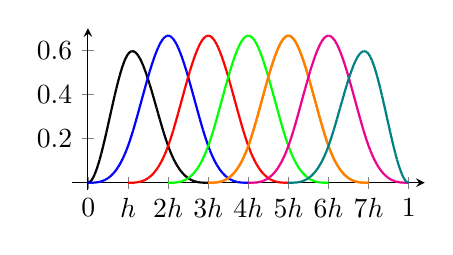
\begin{tikzpicture}
\begin{axis}[xtick={0.001,0.125,0.25,0.375,0.5,0.625,0.75,0.875,1}, 
			 xticklabels={$0$, $h$, $2h$, $3h$, $4h$, $5h$, $6h$, $7h$, $1$}, 
			 axis x line=center, axis y line=center,
			 xmin = 0, xmax = 1, enlargelimits=0.05, 
			 width=0.5\linewidth,
			 height=0.3\linewidth]
			 
\addplot[domain=0:0.125, 
mesh, patch type=cubic spline, patch type sampling,  thick, black]
{-469.3333*x^3 +96.0000*x^2};
\addplot[domain=0.125:0.25,
mesh, patch type=cubic spline, patch type sampling,  thick, black]
{298.6667*(x-0.125)^3 -80.0000*(x-0.125)^2 +2.0000*(x-0.125) +0.5833};
\addplot[domain=0.25:0.375,
mesh, patch type=cubic spline, patch type sampling,  thick, black]
{-85.3333*(x-0.25)^3 +32.0000*(x-0.25)^2 -4.0000*(x-0.25) +0.1667};		 
			
\addplot[domain=0:0.125, 
mesh, patch type=cubic spline, patch type sampling,  thick, blue]
{85.3333*x^3};
\addplot[domain=0.125:0.25,
mesh, patch type=cubic spline, patch type sampling,  thick, blue]
{-256.0000*(x - 0.125)^3 +32.0000*(x - 0.125)^2 +4.0000*(x - 0.125) +0.1667};
\addplot[domain=0.25:0.375,
mesh, patch type=cubic spline, patch type sampling, thick, blue]
{256.0000*(x - 0.25)^3 -64.0000*(x - 0.25)^2 +0.6667};
\addplot[domain=0.375:0.5,
mesh, patch type=cubic spline, patch type sampling,  thick, blue]
{-85.3333*(x - 0.375)^3 +32.0000*(x - 0.375)^2 -4.0000*(x - 0.375) +0.1667};

\addplot[domain=0.125:0.25,
mesh, patch type=cubic spline, patch type sampling,  thick, red]
{85.3333*(x - 0.125)^3};
\addplot[domain=0.25:0.375,
mesh, patch type=cubic spline, patch type sampling,  thick, red]
{-256.0000*(x - 0.25)^3 +32.0000*(x - 0.25)^2 +4.0000*(x - 0.25) +0.1667};
\addplot[domain=0.375:0.5,
mesh, patch type=cubic spline, patch type sampling,  thick, red]
{256.0000*(x - 0.375)^3 -64.0000*(x - 0.375)^2 +0.6667};
\addplot[domain=0.5:0.625,
mesh, patch type=cubic spline, patch type sampling,  thick, red]
{-85.3333*(x - 0.5)^3 +32.0000*(x - 0.5)^2 -4.0000*(x - 0.5) +0.1667};

\addplot[domain=0.25:0.375,
mesh, patch type=cubic spline, patch type sampling,  thick, green]
{85.3333*(x - 0.25)^3};
\addplot[domain=0.375:0.5,
mesh, patch type=cubic spline, patch type sampling,  thick, green]
{-256.0000*(x - 0.375)^3 +32.0000*(x - 0.375)^2 +4.0000*(x - 0.375) +0.1667};
\addplot[domain=0.5:0.625,
mesh, patch type=cubic spline, patch type sampling,  thick, green]
{256.0000*(x - 0.5)^3 -64.0000*(x - 0.5)^2 +0.6667};
\addplot[domain=0.625:0.75,
mesh, patch type=cubic spline, patch type sampling,  thick, green]
{-85.3333*(x - 0.625)^3 +32.0000*(x - 0.625)^2 -4.0000*(x - 0.625) +0.1667};

\addplot[domain=0.375:0.5,
mesh, patch type=cubic spline, patch type sampling,  thick, orange]
{85.3333*(x - 0.375)^3};
\addplot[domain=0.5:0.625,
mesh, patch type=cubic spline, patch type sampling,  thick, orange]
{-256.0000*(x - 0.5)^3 +32.0000*(x - 0.5)^2 +4.0000*(x - 0.5) +0.1667};
\addplot[domain=0.625:0.75,
mesh, patch type=cubic spline, patch type sampling,  thick, orange]
{256.0000*(x - 0.625)^3 -64.0000*(x - 0.625)^2 +0.6667};
\addplot[domain=0.75:0.875,
mesh, patch type=cubic spline, patch type sampling,  thick, orange]
{-85.3333*(x - 0.75)^3 +32.0000*(x - 0.75)^2 -4.0000*(x - 0.75) +0.1667};

\addplot[domain=0.375:0.5,
mesh, patch type=cubic spline, patch type sampling,  thick, orange]
{85.3333*(x - 0.375)^3};
\addplot[domain=0.5:0.625,
mesh, patch type=cubic spline, patch type sampling,  thick, orange]
{-256.0000*(x - 0.5)^3 +32.0000*(x - 0.5)^2 +4.0000*(x - 0.5) +0.1667};
\addplot[domain=0.625:0.75,
mesh, patch type=cubic spline, patch type sampling,  thick, orange]
{256.0000*(x - 0.625)^3 -64.0000*(x - 0.625)^2 +0.6667};
\addplot[domain=0.75:0.875,
mesh, patch type=cubic spline, patch type sampling,  thick, orange]
{-85.3333*(x - 0.75)^3 +32.0000*(x - 0.75)^2 -4.0000*(x - 0.75) +0.1667};

\addplot[domain=0.5:0.625,
mesh, patch type=cubic spline, patch type sampling,  thick, magenta]
{85.3333*(x - 0.5)^3};
\addplot[domain=0.625:0.75,
mesh, patch type=cubic spline, patch type sampling,  thick, magenta]
{-256.0000*(x - 0.625)^3 +32.0000*(x - 0.625)^2 +4.0000*(x - 0.625) +0.1667};
\addplot[domain=0.75:0.875,
mesh, patch type=cubic spline, patch type sampling,  thick, magenta]
{256.0000*(x - 0.75)^3 -64.0000*(x - 0.75)^2 +0.6667};
\addplot[domain=0.875:1,
mesh, patch type=cubic spline, patch type sampling,  thick, magenta]
{-85.3333*(x - 0.875)^3 +32.0000*(x - 0.875)^2 -4.0000*(x - 0.875) +0.1667};

\addplot[domain=0.625:0.75,
mesh, patch type=cubic spline, patch type sampling,  thick, teal]
{85.3333*(x - 0.625)^3};
\addplot[domain=0.75:0.875,
mesh, patch type=cubic spline, patch type sampling,  thick, teal]
{-298.6667*(x - 0.75)^3 +32.0000*(x - 0.75)^2 +4.0000*(x - 0.75) +0.1667};
\addplot[domain=0.875:1,
mesh, patch type=cubic spline, patch type sampling,  thick, teal]
{469.3333*(x - 0.875)^3 -80.0000*(x - 0.875)^2 -2.0000*(x - 0.875) +0.5833};


\end{axis}
\end{tikzpicture}

\end{document}